\documentclass[12pt]{article}

\newcommand{\CiteMathPackage}{../../math}
\newcommand{\CiteReference}{../reference.bib}

% Packages
\usepackage{setspace,geometry,fancyvrb,rotating}
\usepackage{marginnote,datetime,enumitem}
\usepackage{titlesec,indentfirst}
\usepackage{amsmath,amsfonts,amssymb,amsthm,mathtools}
\usepackage{threeparttable,booktabs,adjustbox}
\usepackage{graphicx,epstopdf,float,soul,subfig}
\usepackage[toc,page]{appendix}
\usdate

% Page Setup
\geometry{scale=0.8}
\titleformat{\paragraph}[runin]{\itshape}{}{}{}[.]
\titlelabel{\thetitle.\;}
\setlength{\parindent}{10pt}
\setlength{\parskip}{10pt}
\usepackage{Alegreya}
\usepackage[T1]{fontenc}

%% Bibliography
\usepackage{natbib,fancybox,url,xcolor}
\definecolor{MyBlue}{rgb}{0,0.2,0.6}
\definecolor{MyRed}{rgb}{0.4,0,0.1}
\definecolor{MyGreen}{rgb}{0,0.4,0}
\definecolor{MyPink}{HTML}{E50379}
\newcommand{\highlightR}[1]{{\emph{\color{MyRed}{#1}}}} 
\newcommand{\highlightB}[1]{{\emph{\color{MyBlue}{#1}}}}
\newcommand{\highlightP}[1]{{\emph{\color{MyPink}{#1}}}}
\usepackage[bookmarks=true,bookmarksnumbered=true,colorlinks=true,linkcolor=MyBlue,citecolor=MyRed,filecolor=MyBlue,urlcolor=MyGreen]{hyperref}
\bibliographystyle{econ}

%% Theorem Environment
\theoremstyle{definition}
\newtheorem{assumption}{Assumption}
\newtheorem{definition}{Definition}
\newtheorem{theorem}{Theorem}
\newtheorem{proposition}{Proposition}
\newtheorem{lemma}[theorem]{Lemma}
\newtheorem{example}{Example}
\newtheorem{corollary}[theorem]{Corollary}
\usepackage{mathtools}
\usepackage{\CiteMathPackage}


\begin{document}


%??%??%??%??%??%??%??%??%??%??%??%??%??%??%??%??%??%??%??%??%??%??
%?? title
%??%??%??%??%??%??%??%??%??%??%??%??%??%??%??%??%??%??%??%??%??%??

\title{\bf The Race between Man and Machine: Implications of Technology for Growth, Factor Shares, and Employment, American Economic Review, 2018}
\author{Wenzhi Wang \thanks{This note is written in my pre-doc period at the University of Chicago Booth School of Business.} } 
\date{\today}
\maketitle

\citet{acemogluRaceManMachine2018}

\section{The Static Model}

We start with a static version of our model with exogenous technology, which allows us to introduce our main setup in the simplest fashion and characterize the impact of different types of technological change on factor prices, employment, and the labor share.

\subsection{Environment}

The economy produces a unique final good $Y$ by combining a unit measure of tasks, $y\of{i}$, with an elasticity of substitution $\sigma \in \bp{0, \infty}$:
\begin{equation}
    \label{eq: overall_production_function}
	Y = \widetilde{B}\left(\int_{N-1}^N y(i)^{\frac{\sigma-1}{\sigma}} d i\right)^{\frac{\sigma}{\sigma-1}}
\end{equation}
where $\wt{B} > 0$. All tasks and the final good are produced competitively. The fact that the limits of integration run between $N-1$ and $N$ imposes that the measure of tasks used in production always remains at $1$. A new (more complex) task replaces or upgrades the lowest-index task. Thus, an increase in $N$ represents the upgrading of the quality (productivity) of the unit measure of tasks.

Each task is produced by combining labor or capital with a task-specific intermediate $q\of{i}$, which embodies the technology used either for automation or for production with labor. We start by assuming that these intermediates are supplied competitively, and that they can be produced using $\psi$ units of the final good. Hence, they are also priced at $\p$. In later Section we relax this assumption and allow intermediate producers to make profits so as to generate endogenous incentives for innovation.

All tasks can be produced with labor. We model the technological constraints on automation by assuming that there exists $I \in \bs{N-1, N}$ such that tasks $i \leq I$ are \highlightB{technologically automated} in the sense that it is feasible to produce them with capital. Although tasks $i \leq I$ are technologically automated, whether they will be produced with capital or not depends on relative factor prices as we describe below. Conversely, tasks $i>I$ are not technologically automated, and must be produced with labor.

The production function for tasks $i > I$ takes the form
\begin{equation} 
    \label{eq: complex_task_production_function}
	y(i) = \ol{B}(\zeta)\left[\eta^{\frac{1}{\zeta}} q(i)^{\frac{\zeta-1}{\zeta}}+(1-\eta)^{\frac{1}{\zeta}}(\gamma(i) l(i))^{\frac{\zeta-1}{\zeta}}\right]^{\frac{\zeta}{\zeta-1}},
\end{equation}
where $\gamma\of{i}$ denote the productivity of labor in task $i$, $\zeta \in \bp{0, \infty}$ is the elasticity of substitution between intermediates and labor, $\eta \in \bp{0,1}$ is the share parameter of this CES production function, and $\ol{B}(\zeta)$ is a constant, $\ol{B}(\zeta) = \psi^\eta(1-\eta)^{\eta-1} \eta^{-\eta}$ when $\zeta=1$, and $\ol{B}(\zeta)=1$ otherwise.

Tasks $i \leq I$ can be produced using labor or capital, and their production function is identical to (\ref{eq: complex_task_production_function}) expect for the presence of capital and labor as perfectly substitutable factors of production:
\begin{equation}
    \label{eq: simple_task_production_function}
	y(i) = \ol{B}(\zeta)\left[\eta^\frac{1}{\zeta} q(i)^{\frac{\zeta-1}{\zeta}}+(1-\eta)^\frac{1}{\zeta}(k(i)+\gamma(i) l(i))^{\frac{\zeta-1}{\zeta}}\right]^{\frac{\zeta}{\zeta-1}}
\end{equation}

Throughout, we impose the following assumption.
\begin{assumption}
    \label{assumption_1}
	$\gamma\of{i}$ is strictly increasing.
\end{assumption}
It implies that labor has strict \highlightB{comparative advantage} in tasks with a higher index and will guarantee that, in equilibrium, tasks with lower indices will be automated, while those with higher indices will be produced with labor.

We model the demand side of the economy using a representative household with preferences given by
\begin{equation}
    \label{eq: utility_function}
	u(C, L) = \frac{\left(C e^{-\nu(L)}\right)^{1-\theta}-1}{1-\theta},
\end{equation}
where $\nu\of{L}$ designates the utility cost of labor supply, which we assume to be continuously differentiable, increasing, and convex, and to satisfy $\nu^{\prime\prime}\of{L} + \bp{\t-1}\times\bp{\nu^{\prime}\of{L}}^2 / \t > 0$ (which ensures that $u\of{C, L}$ is concave). This functional form in (\ref{eq: utility_function}) ensures balanced growth. When we turn to the dynamic analysis in the next Section, $\t$ will be the inverse of the intertemporal elasticity of substitution.

Finally, in the static model, the capital stock, $K$, is taken as given.

\subsection{Equilibrium in the Static Model}

Given the set of technologies $I$ and $N$, and the capital stock $K$, we now characterize the equilibrium value of output, factor prices, employment, and the threshold task $I^*$.

In the text, we simplify the exposition by imposing the following assumption.
\begin{assumption}
    \label{ass_2}
	One of the following two conditions holds:
	\begin{itemize}[topsep=0pt, leftmargin=30pt, itemsep=0pt]
		\setlength{\parskip}{10pt} 
		\item $\cvg{\eta}{0}$, or
		\item $\zeta = 1$.
	\end{itemize}
\end{assumption}

\highlightP{These two special cases ensure that the demand for labor and capital is homothetic.} More generally, our qualitative results are identical as long as the degrees of non-homotheticity is not too extreme, though in this case we no longer have closed-form expressions.

%todo
\highlightP{How can I derive this unit cost of production?}

We proceed by characterizing the unit cost of producing each task as a function of factor prices and the automation possibilities represented by $I$. Because tasks are produced competitively, their price, $p\of{i}$, will be equal to the minimum unit cost of production:
\begin{equation}
    \label{eq: price_of_tasks}
	p(i)=\left\{\begin{array}{ll}
		\min \left\{R, \frac{W}{\gamma(i)}\right\}^{1-\eta} & \text { if } i \leq I \\
		\left(\frac{W}{\gamma(i)}\right)^{1-\eta} & \text { if } i>I
	\end{array},\right.
\end{equation}
where $W$ denotes the wage rate and $R$ denotes the rental rate of capital. In Equation (\ref{eq: price_of_tasks}), the unit cost of production for tasks $i > I$ is given by the effective cost of labor, $W / \g\of{i}$ (which takes into account that the productivity of labor in task $i$ is $\g\of{i}$). The unit cost of production for tasks $i \leq I$ is given by $\min \left\{R, \frac{W}{\gamma(i)}\right\}^{1-\eta}$, which reflects the fact that capital and labor are perfect substitutes in the production of automated tasks. In these tasks, firms will choose whichever factor has a lower effective cost: $R$ or $W /\g\of{i}$.

Because labor has a strict comparative advantage in tasks with a higher index, there is a (unique) threshold $\wt{I}$ such that 
\begin{equation}
    \label{eq: endogenous_task_threshold}
	\frac{W}{R} = \gamma\of{\wt{I}}.
\end{equation}
This threshold represents the task for which the costs of producing with capital and labor are equal. Combing with our constraint imposed by the available automation technology, this implies that there exists a unique equilibrium threshold task $$I^* = \min \bc{I, \wt{I}},$$such that all tasks $i \leq I^*$ will be produced with capital, while all tasks $i > I^*$ will be produced with labor.

Figure \ref{fig: task_space} depicts the resulting allocation of tasks to factors and also shows how, as already noted, the creation of new tasks replaces existing tasks from the bottom of the distribution. 

\begin{figure}[H]
	\noindent\caption{The Task Space and a Representation of the Effect of Introducing New Tasks (Panel B) and Automating Existing Tasks (Panel C)}
	\centerline{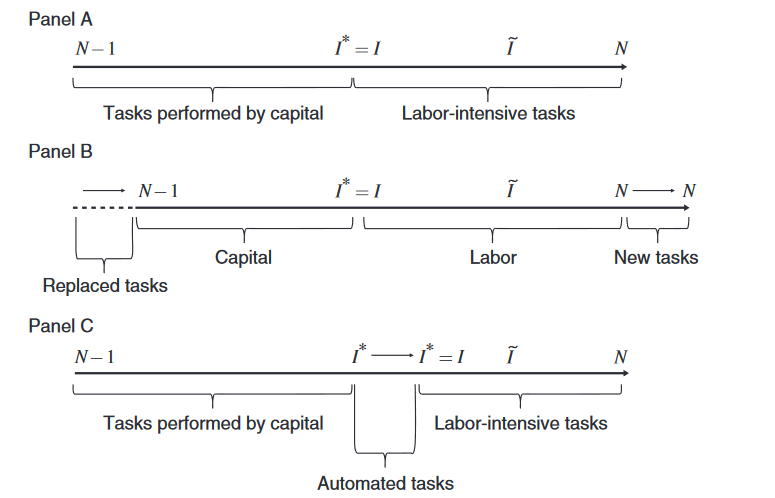
\includegraphics[scale=0.9]{acemoglu2018_fig2.png}}
    \label{fig: task_space}
\end{figure}

Since we have simplified the exposition by imposing that new tasks created at $N$ immediately replace tasks located at $N-1$, and it is therefore profitable to produce new tasks with labor (and hence we have not distinguished $N$, $N^*$, and $\wt{N}$). In the static model, this will be the case when the capital stock is not too large, which is imposed in the next Assumption.

\begin{assumption}
    \label{ass_3}
	We have $K  < \ol{K}$, where $\ol{K}$ is such that $R = \frac{W}{\gamma\of{N}}$.
\end{assumption}
This assumption ensures that $R > \frac{W}{\gamma\of{N}}$, and consequently, new tasks will increase aggregate output and will be adopted immediately. Outside of this region, new tasks would not be utilized, which we view as the less interesting case. This Assumption is relaxed in the next two Sections where the capital stock is endogenous.

We next derive the demand for factors in terms of the (endogenous) threshold $I^*$ and the technology parameter $N$. We choose the final good as the numeraire. Equation (\ref{eq: overall_production_function}) gives the demand for task $i$ as 
\begin{equation}
    \label{eq: demand_for_task_i}
    y\of{i} = \wt{B}^{\s - 1} Y p\of{i}^{-\s}.
\end{equation}

Let us define $\wh{\s} = \s\bp{1 - \eta} + \zeta \eta$ and $B = \wt{B}^{\frac{\s-1}{\wh{\s}-1}}$. Under Assumption \ref{ass_2}, Equations (\ref{eq: complex_task_production_function}) and (\ref{eq: simple_task_production_function}) yield the demand for capital and labor in each task as 
\begin{equation}
    \notag 
    k(i)= \begin{cases}B^{\widehat{\sigma}-1}(1-\eta) Y R^{-\widehat{\sigma}} & \text { if } i \leq I^* \\ 0 & \text { if } i>I^*\end{cases}
\end{equation}
and 
\begin{equation}
    \notag 
    l(i)= \begin{cases}0 & \text { if } i \leq I^* \\ B^{\widehat{o}-1}(1-\eta) Y \frac{1}{\gamma(i)}\left(\frac{W}{\gamma(i)}\right)^{-\widehat{o}} & \text { if } i>I^*\end{cases} .
\end{equation}

We can now define a \highlightB{static equilibrium} as follows. Given a range of tasks $\bs{N-1, N}$, automation technology $I \in (N-1, N]$, and a capital stock $K$, a static equilibrium is summarized by a set of factor prices, $W$ and $R$, threshold tasks, $\wt{I}$ and $I^*$, employment level, $L$, and aggregate output $Y$, such that 
\begin{itemize}[topsep=0pt, leftmargin=20pt, itemsep=0pt]
\setlength{\parskip}{10pt} 
\item $\wt{I}$ is determined by Equation (\ref{eq: endogenous_task_threshold}) and $I^* = \min \bc{I, \wt{I}}$;

\item The capital and labor market clear, so that 
\begin{equation}
    \label{eq: capital_market_clear}
    B^{\widehat{\sigma}-1}(1-\eta) Y\left(I^*-N+1\right) R^{-\widehat{\sigma}}=K ,
\end{equation}
\begin{equation}
    \label{eq: labor_market_clear}
    B^{\widehat{\sigma}-1}(1-\eta) Y \int_{I^*}^N \frac{1}{\gamma(i)}\left(\frac{W}{\gamma(i)}\right)^{-\widehat{\sigma}} d i=L ;
\end{equation}

\item Factor prices satisfy the \highlightB{ideal price index condition},
\begin{equation}
    \label{eq: ideal_price_index_condition}
    \left(I^*-N+1\right) R^{1-\widehat{\sigma}}+\int_{I^*}^N\left(\frac{W}{\gamma(i)}\right)^{1-\widehat{\sigma}} d i=B^{1-\widehat{\sigma}}
\end{equation}

\item Labor supply satisfies $\nu^\prime\of{L} = W / C$. Since in equilibrium $C = RK + WL$, this condition can be rearranged to yield the following increasing labor supply function:
\begin{equation}
    \label{eq: labor_supply_function}
    L=L^s\left(\frac{W}{R K}\right)
\end{equation}
\end{itemize}

\begin{proposition}[Equilibrium in the Static Model]
    \label{prop_1}
    Suppose that Assumptions \ref{assumption_1}, \ref{ass_2}, and \ref{ass_3} hold. Then a static equilibrium exists and is unique. In this static equilibrium, aggregate output is given by 
    \begin{equation}
        \label{eq: aggregate_output}
        Y=\frac{B}{1-\eta}\left[\left(I^*-N+1\right)^{\frac{1}{\sigma}} K^{\frac{\hat{\sigma}-1}{\hat{\sigma}}}+\left(\int_{I^*}^N \gamma(i)^{\hat{\sigma}-1} d i\right)^{\frac{1}{\hat{\sigma}}} L^{\frac{\hat{\sigma}-1}{\hat{\sigma}}}\right]^{\frac{\widehat{\sigma}}{\hat{\sigma}-1}} .
    \end{equation}
\end{proposition}

Equation (\ref{eq: aggregate_output}) shows that the aggregate output is a CES aggregate of capital and labor, with the elasticity between capital and labor being $\wh{\s}$. The share parameters are endogenous and depend on the state of the two types of technologies and the equilibrium choices of firms. An increase in $I^*$, which corresponds to greater equilibrium automation, increases the share of capital and reduces the share of labor in this aggregate production function, while the creation of new tasks does the opposite.

\begin{figure}[H]
    \noindent\caption{Static Equilibrium}
    \begin{center}
        \resizebox{0.7\textwidth}{!}{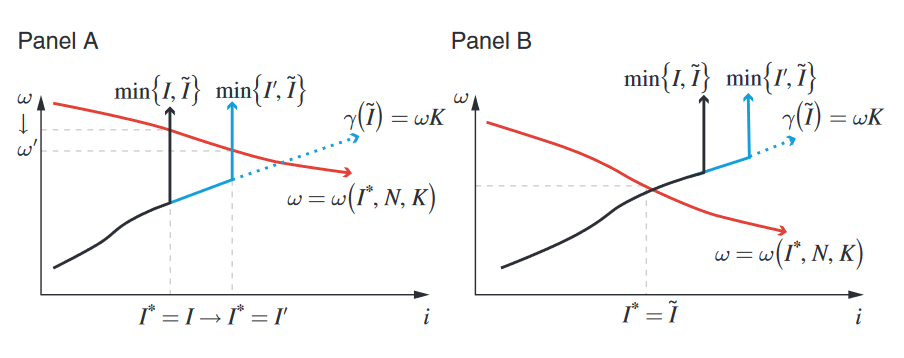
\includegraphics{acemoglu2018_fig3.png}}
    \end{center}
    % \smallskip
    {\footnotesize Notes: Panel A depicts the case in which $I^* = I < \wt{I}$ so that the allocation of factors is constrained by technology. Panel B depicts the case in which $I^* = \wt{I} < I$ so that the allocation of factors is not constrained by technology and is cost-minimizing. The blue curves show the shifts following an increase in $I$ to $I^\prime$, which reduce $\o$ in the panel A, but have no effect in panel B.}
    \label{fig: static_equilibrium}
\end{figure}

Figure \ref{fig: static_equilibrium} illustrates the unique equilibrium described in Proposition \ref{prop_1}. The equilibrium is given by the interaction of two curves in the $\bp{\o, I}$ space, where $\o = \frac{W}{RK}$ is the wage level normalized by capital income; this ratio is a monotone transformation of the labor share and will play a central role in the rest of our analysis. THe upward-sloping curve represents the cost-minimizing allocation of capital and labor to tasks represented by Equation (\ref{eq: endogenous_task_threshold}), with the constraint that the equilibrium level of automation can never exceed $I$. The downward-sloping curve, $\o\of{I^*, N, K}$, corresponds to the relative demand for labor, which can be obtained directly from (\ref{eq: capital_market_clear}), (\ref{eq: labor_market_clear}), and (\ref{eq: labor_supply_function}) as 
\begin{equation}
    \label{eq: normalized_wage_income}
    \ln \omega+\frac{1}{\widehat{\sigma}} \ln L^s(\omega)=\left(\frac{1}{\widehat{\sigma}}-1\right) \ln K+\frac{1}{\widehat{\sigma}} \ln \left(\frac{\int_{L^*}^N \gamma(i)^{\widehat{\sigma}-1} d i}{I^*-N+1}\right).
\end{equation}
As we show in Appendix A, the relative demand curve always starts above the cost minimization condition and ends up below it, so that the two curves necessarily intersect, defining a unique equilibrium as shown in Figure \ref{fig: static_equilibrium}.

Figure \ref{fig: static_equilibrium} also distinguishes between the two cases highlighted above. In Panel A, we have $I^* = I < \wt{I}$ and the allocation of factors is constrained by technology, while Panel B plots the case where $I^* = \wt{I} < I$ and firms choose the cost-minimizing allocation given factor prices.

A special case of Proposition \ref{prop_1} is also worth highlighting, because it leads to a Cobb-Douglas production function with an exponent depending on the degree of automation, which is particularly tractable in certain applications.

\begin{corollary}
    Suppose that $\s = \zeta = 1$, and $\g\of{i} = 1$ for all $i$. Then aggregate output is 
    $$
    Y = \frac{B}{1 - \eta} K^{1 - N + I^*} L^{N - I^*}.
    $$
\end{corollary}

The next two propostions give a complete characterization of comparative statics. 




\section{Dynamics and Balanced Growth}

In this Section, we extend our model to a dynamic economy in which the evolution of the capital stock is determined by the saving decisions of a representative household. We then investigate the conditions under which the economy admits a balanced growth path (BGP), where aggregate output, the capital stock, and wages grow at a constant rate. We conclude by discussing the long-run effects of automation on wages, the labor share, and employment. 

\subsection{Balanced Growth}



\bibliography{\CiteReference}


\end{document}